\chapter{LPWAN e Lora}
Nel seguente capitolo si approfondirà il concetto di rete \emph{LPWAN} e la sua
struttura, andando ad analizzare i vari layer di cui è composta. 
In particolare si farà riferimento alla tecnologia Lora che implementa questo
tipo di rete, andandone ad analizzare i vari componenti, quali
\begin{itemize}
\item layer fisico
\item la composizione dei pachetti 
\item le classi di devices implementati
\end{itemize}

\section{LPWAN}
Tra le varie tipologie di rete emergenti per l'IoT, LPWAN sta riscuotendo sempre
più interesse. Questo tipo di rete si basa sulla topologia a stella, la quale
permette di avere un elevato numero di devices connessi ad una sola stazione
base.Inoltre per la sua struttura LPWAN supporta comunicazioni a lungo raggio
risultando adatta per i vari \emph{use-case} del internet of things. I due
principali concorrenti che implementano queste tecnologie sono Sigfox\tm e
Semtech\tm possessore di Lora\tm. L'implementazione proposta da Sigfox utilizza
la Ultra Narrow Band tramite la quale è possibili inviare messaggi con payload
lungo 12 \emph{byte} in 6 secondi usando una frequenza di 100[Hz]. Per via delle
varie regolazioni, utilizzando la tecnologia Sigfox si ha un numero limitato di
messaggi per giorno.
Al contrario la tecnologia Lora, implementa \emph{spread spectrum Physical
Layer} (PHY) il quale permette una maggiore ricezione andando ad influire sul
data-rate possibile

\section{Lora}
\emph{Lora} è una tecnologia semi-proprietaria, sviluppata da Semtech. Lora è
composta da un parte proprietaria detta \emph{Lora}\cite{LoRaCss101} la quale definisce il layer
fisico, e una parte libera chiamata LoRaWAN\cite{LoRaWAN101}.
\improvement[inline]{Completare e riscrivere}


\section{CSS}
Alla base del layer fisico troviamo la modulazione (CSS), questo tipo di
modulazione della frequenza, utilizzata anche in altre applicazioni radio, 
esempio radar ecc..\improvement{Aggiungere qualche altro esempio}.
Questo tipo di modulazione ha numerosi vantaggi quali 
\begin{itemize}
\item Uno spettro idealmente rettangolare, il quale utilizza tutta la capacità
del canale e fornisce un ottima densità spettrale di potenza rispetto agli atri
tipi di trasmissione.
\item \textbf{Segnali di tipo Chirp} possono essere sovrapposti in modo tale da
poter variare il data-rate e l'energia per bit in modo adattativo per aumentare
l'efficienza complessiva.
\item \textbf{Hanno guadagno programmabile}, il quale permette di raggiungere
distanze considerevoli mantenendo un buon SNR .
\item  \textbf{Ottima risoluzione nel asse del tempo}, quindi ottimi per coprire
lunghe distanze.
\item \textbf{Immuni al effetto Doppler} 
\item \textbf{Immuni al degenerazioni per effetto di multipath} \info{Trovare
termine per multipath}
\end{itemize}
Un segnale di tipo \emph{Chirp} assume valori compresi nella banda di frequenza
$B = [f_0,f_1]$, il suo andamento è di tipo monotono , crescente o decrescente
compreso tra le due frequenze $f_0$ e $f_1$.

\begin{figure}
\begin{subfigure}[h]{\textwidth}
\centering
\import{Images/Eps/}{Chirp.eps_tex}
\caption{Segnale Chirp nel dominio della frequenza}
\end{subfigure}

\begin{subfigure}[h]{\textwidth}
\centering
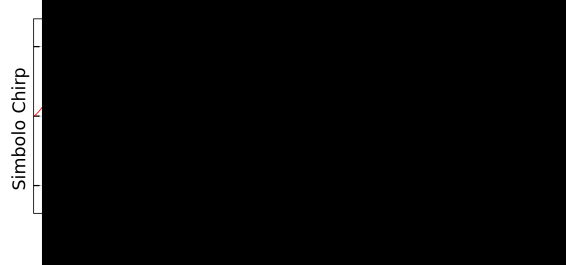
\includegraphics[width=\textwidth]{Time_Chirp}
\caption{Simbolo codificato col metodo Chirp nel dominio del tempo}
\end{subfigure}
\end{figure}

Uno degli aspetti principali del layer fisico, è la possibilità di adattare il
numero di bit codificati in un simbolo in base alle varie esigenze. Questa
possibilità\info{Riscrivere} di adattamento permette a parità di potenza di
riuscire a raggiunger distanze maggiori andando a variare, quello che nella
documentazione ufficiale è chiamato \emph{Spread Factor}. Tutto ciò significa
che (SF) rappresenta $2^{\text{SF}}$ bits in un simbolo. Un differente SF
implica anche un differente tempo di comunicazione secondo la formula
\begin{equation}
        T_s=\frac{2^{\text{SF}}}{B}.
\end{equation}

Dalla quale si evince che andando ad aumentare lo spread factor di una unità,
mantenendo una lunghezza di banda fissa $B$, otteniamo un raddoppio nel tempo di
trasmissione. Il fatto di avere messaggi più lunghi, conferisce un robustezza
superiore alle interferenze e al rumore. In discapito a tutto ciò, il fatto di
dover codificare il messaggio con un maggiore numero di simboli, aumenta la
possibilità di errore alla ricezione. 

\begin{figure}[h]
\centering 
\import{Images/Eps/}{Chirp_SF.eps_tex}
\caption{Comparazione simbolica dei vari SF}
\end{figure}

Questa nuovo modo di trasmettere i vari dati porta con se molti vantaggi.
\begin{itemize}
\item La modulazione Lora è semplice da implementare nei dispositivi, quindi i
moduli radio al loro interno saranno economici.
\item Resistente alle interferenze in banda e fuori banda.
\item Resistente  all'effetto Doppler, in questo modo è possibili utilizzare
cristalli non molto accurati al interno dei devices, in modo tale da abbattere i
costi di produzione.
\item Il modulo di ricezione è altrettanto semplice da costruire, quindi non
molto costoso.
\end{itemize}
\improvement{Rivedere i vari punti e cambiare il linguaggio}

Analizzando lo spettrogramma di una comunicazione Lora è possibili fare delle
osservazioni interessanti. 

\begin{figure}[h]
\centering 
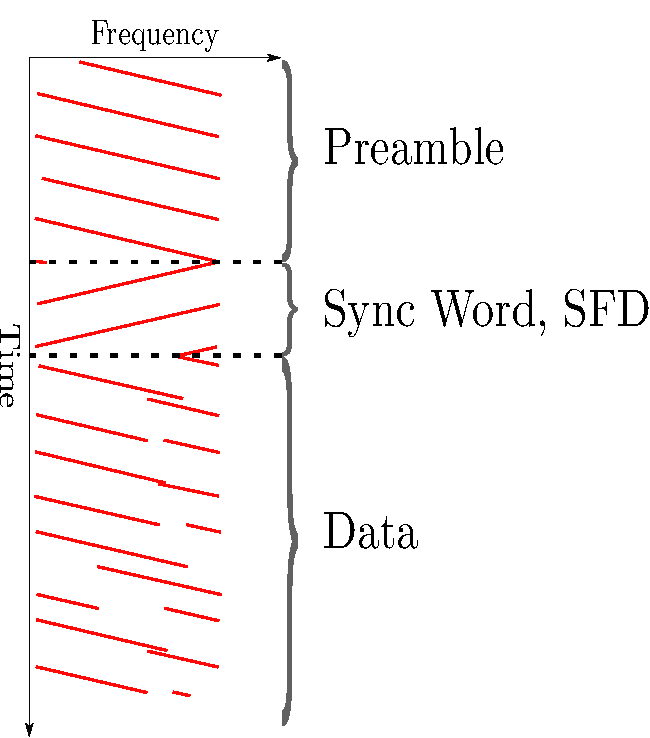
\includegraphics[width=9cm]{Chirp_Message}
\caption{Struttura pacchetto Lora }
\end{figure}

Le varie parti del pacchetto  sono facilmente determinabili, infatti e facile
vedere che il preambolo è codificato con una serie di \emph{Up-chirp}, il quale
finito inizia una serie di \emph{down-chirp} i quali determinano il SFD o Header
il quale contiene informazioni aggiuntive e possibilmente dei bit per il
controllo e correzione degli errori\unsure{Controllare header pacchetto}.
\improvement[inline]{Aggiungere immagine e finire la spiegazione}

Per quanto riguarda la struttura interna dei moduli radio, non si hanno molte
informazioni dato che la tecnologia è proprietaria di Semtech. Nella
documentazione ufficiale è presente uno schema a blocchi il quale illustra i
vari blocchi presenti al interno dei moduli radio
\begin{figure}[h]
\centering 
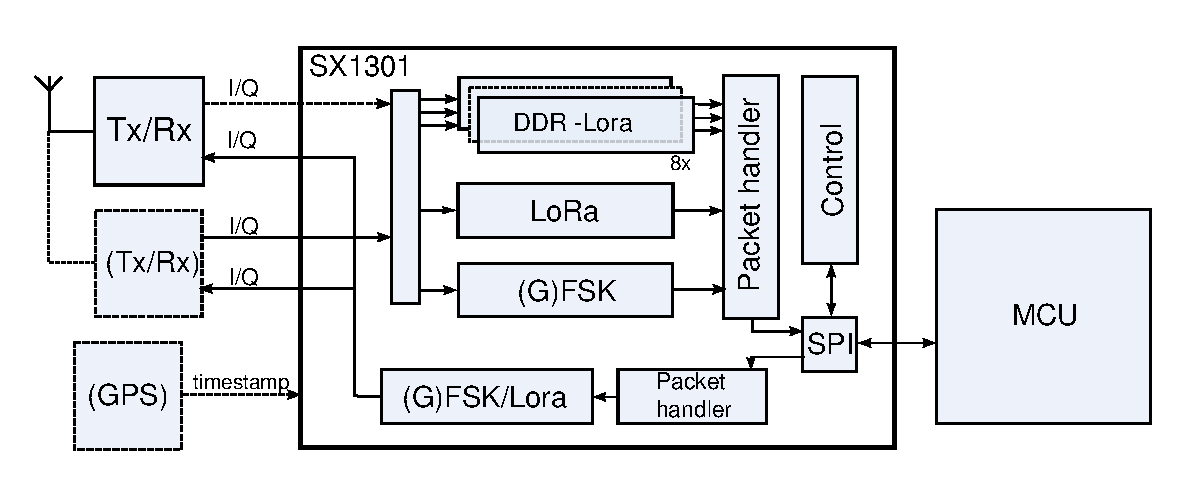
\includegraphics[width=11cm]{SX1301}
\caption{Struttura interna ricevitore SX1301}
\end{figure}
Come possiamo vedere, il gateway rimane in ascolto su 8 frequenze diverse, le
quali permettono di coprire tutti i vari SF. Questo tipo di ricevitore può
demodulare fino ad un massimo di 8 pacchetti contemporaneamente. Inoltre questa
topologia permette di avere vari vantaggi
\begin{itemize}
\item I vari nodi della rete, possono cambiare frequenza in ogni trasmissione in
modo casuale, andando a migliorare di molto la robustezza del sistema alle varie
interferenze.
\item Non è necessario avere tabelle contenenti informazioni riguardanti il
datarate dei vari nodi. Ogni datarate viene demodulato contemporaneamente.
\end{itemize}
\unsure{Riguardare e aggiungere ultimo punto della documentazione pagina 14}

